\documentclass[12pt,a4paper]{report}
\usepackage[utf8]{inputenc}
\usepackage[T1]{fontenc}
\usepackage[spanish]{babel}
\usepackage{graphicx}
\usepackage{enumitem}
\usepackage{fancyhdr}
\usepackage[a4paper, top=3cm, bottom=2.5cm, left=3.5cm, right=3cm]{geometry}
\usepackage[hidelinks]{hyperref}
\usepackage{xcolor}
\usepackage{tabularx}
\usepackage{url}


% Definir el color personalizado
\definecolor{myblue}{HTML}{74EDFF}


\title{Trabajo de Fin de Máster: [Título del TFM]}
\author{José Enrique Rodríguez González}
\date{Enero de 2024}

\geometry{headheight=2cm}

% Configuración de los estilos de página con fancyhdr
\pagestyle{fancy}
\fancyhf{} % Limpia los encabezados y pies de página existentes
\rhead{
\includegraphics[width=\textwidth,height=1.5cm,keepaspectratio]{imagenes/002-imagen-cabecera.png}} % Utiliza una imagen de ejemplo
\renewcommand{\headrulewidth}{0pt} % Elimina la línea del encabezado
\renewcommand{\footrulewidth}{3pt} % Grosor de la línea del pie de página
\renewcommand{\footrule}{\hbox to\headwidth{\color{myblue}\leaders\hrule height \footrulewidth\hfill}} % Color de la línea
\fancyfoot[L]{M1.881 - TFM - Análisis forense} % Texto a la izquierda en el pie de página
\fancyfoot[R]{\thepage} % Número de página a la derecha en el pie de página

\fancypagestyle{plain}{
    \rhead{
\includegraphics[width=\textwidth,height=1.5cm,keepaspectratio]{imagenes/002-imagen-cabecera.png}}
    \rfoot{\thepage}
}


\begin{document}

\pagenumbering{roman}

\begin{titlepage}
    \begin{center}
        \Huge \textbf{Análisis forense de un ordenador personal}
    \end{center}

    \vspace{1cm} % Ajusta el espacio vertical como prefieras

    \begin{minipage}{0.5\textwidth}
        
\includegraphics[width=0.8\textwidth]{imagenes/001-imagen-portada.png} % reemplaza 'example-image' por el nombre de tu imagen
    \end{minipage}
    \begin{minipage}{0.5\textwidth}
        \textbf{Alumno:} \\
        {José Enrique Rodríguez González} \\
        \\
        \textbf{Master Universitario de Ciberseguridad y privacidad.} \\
        \\
        \textbf{M1.881 - TFM - Análisis forense} \\
        \\
        \textbf{Tutora de TFM:} \\
        {Dña. Elena Botana de Castro} \\
        \\
        \textbf{Profesor responsable de la asignatura:} \\
        {D. Jordi Serra Ruiz} \\
        \\
        \textbf{Fecha de Entrega:} \\
        {Enero de 2024}
    \end{minipage}

    \vfill % Llena el espacio vertical para empujar el siguiente contenido hacia abajo

    % Otro contenido que quieras poner en tu portada

\end{titlepage}
\restoregeometry


\newpage  % Crear una nueva página


\addcontentsline{toc}{chapter}{Deuda técnica}  % Añadir a la Tabla de Contenidos
\chapter*{Deuda técnica}  % Crear un capítulo sin número

Este no es un capitulo al uso del TFM, si no que tratará de llevar un control de las tareas pendientes (Deuda técnica) de todo el TFM.

PEC 1

\begin{enumerate}
    \item {\color{red}\textbf{DEUDA TÉCNICA: Pendiente de Referenciar!!!, enunciado del TFM}}
    \item {\color{red}\textbf{DEUDA TÉCNICA: Pendiente de Referenciar!!!, referenciar de la web de los TFM}}
    \item {\color{red}\textbf{DEUDA TÉCNICA: Buscar presidente de los EE.UU., preguntar a "//4lanoga"}}
    
    {\color{red}\textbf{LA RESPUESTA ES REAGAN}}
    
    \item {\color{red}\textbf{DEUDA TÉCNICA: Listado de aplicaciones a utilizar en la descripción del entorno de trabajo}}
    \item {\color{red}\textbf{DEUDA TÉCNICA: plantear posible reducción del estado del arte}}
    \item {\color{red}\textbf{DEUDA TÉCNICA: Referencia a WIKIPEDIA}}
    
\end{enumerate}
\clearpage


\addcontentsline{toc}{chapter}{Agradecimientos}  % Añadir a la Tabla de Contenidos
\chapter*{Agradecimientos}  % Crear un capítulo sin número
A mi esposa e hija, acompañantes en todo momento de esta aventura académida.

A mis compañeros de trabajo, Juanma, Luisma y Borja, que saben de que estos tres años que llevo realizando este master y han conocido todos los derroteros que me ha llevado este camino.
\clearpage

\tableofcontents % Crea el índice

\newpage
\pagenumbering{arabic}

\chapter{Plan de trabajo.}
esto es parte del texto del plan de trabajo % Importa el contenido del archivo 002-plan-de-trabajo.tex
\clearpage

\section{Problema a resolver.}
Por, lo expuesto en la introducción del capítulo, se coliga que el problema a resolver es la resolución de las cuestiones solicitadas por el Gerente de la empresa.

Una definición idónea que se puede adoptar en el presente TFM es lo indicado en su momento en la propuesta del TFM:

Solventar las necesidades del gerente de la empresa mediante el análisis forense del disco duro y la captura de memoria de un ordenador personal, en un caso real con un sistema virtualizado, vinculado a una presunta conducta delictiva real. Para ello, se utilizarán herramientas específicas para la localización de las evidencias digitales sobre los discos duros y la memoria que puedan demostrar el presunto delito (Encase, Autopsy, Volatility, o cualquier otra herramienta, o conjunto de herramientas con prestaciones equivalentes). Finalmente, las evidencias localizadas deberán recogerse en un informe ejecutivo o pericial, el cual, además de los aspectos técnicos, deberá tener en cuenta aquellos requisitos procesales necesarios para que el análisis pueda tener validez en un proceso judicial.

{\color{red}\textbf{DEUDA TÉCNICA: Pendiente de Referenciar!!!, referenciar de la web de los TFM}}
\clearpage

\section{Objetivos.}
Se describe un el siguiente listado de objetivos que se obtienen al analizar el enunciado del TFM:

\begin{enumerate}
    \item Elaboración del Análisis forense de Disco Duro y RAM.
    \begin{enumerate}
        \item realizar una recuperación parcial o total de la información borrada existente en los dispositivos susceptibles de ser analizados (carving).
        \item Relativo al análisis de la memoria RAM. 
        \begin{enumerate}
            \item Comprobar la integridad de la memoria RAM.
            \item Comprobar fecha de la captura de la RAM.
            \item Determinar la edición y versión de Windows que tiene instalado el sistema operativo del ordenador sobre el cual se ha efectuado la captura de la memoria RAM.
            \item Buscar los procesos en funcionamiento y localiza aquellos que te parezcan de interés para el análisis forense del ordenador analizado.
            \item Extraer los procesos que consideres sospechosos y analízarlos.
            \item Listar las conexiones de red y analizarlas.
        \end{enumerate}
        \item Relativo al analisis del Disco Duro. 
        \begin{enumerate}
            \item Comprobar la integridad del disco duro.
            \item Determinar la siguiente información del disco duro.
            \begin{enumerate}
                \item Tamaño del disdo duro analizado.
                \item Sistema y versión del sistema operativo instalado.
                \item Nombre del propietario y relación de software instalado.
                \item “Product ID” y “Product Key” asociadas al sistema.
                \item Fecha y hora de instalación del sistema operativo.
                \item Determinar marca y modelo (si es posible) del hardware siguiente: CPU, monitor, tarjeta gráfica, tarjeta Ethernet y Wireless.
            \end{enumerate}
            \item Determinar qué usuarios tiene definidos el sistema.
            \item Localizar los documentos (archivos PDF, de texto, hojas de cálculo, etc.) que puedan tener relación con alguna conducta presuntamente delictiva.
            \item Localizar los archivos eliminados y determina si hay alguno relevante para la causa investigada.
            \item Localizar los ficheros comprimidos relevantes analizarlos, reventar contraseña si es necesario y analizar su contenido.
            \item Localizar algún fichero ejecutable que pueda resultar de interés para la investigación, ademas, analizar la relacion con alguna evidencia anterior.
            \item Determinar el contenido del fichero log de un conocido programa de comunicación si es necesario y relaciónarlo con el caso investigado.
            \item Realizar un analisis de la navegacion web.
            \item Estudio de los dispositivos físicos que en algún momento fueron conectados al sistema estudiado: móviles, USBs, impresoras, escáneres, cámaras, tarjetas de memoria.
            \item Estudio de la información contenida en los unallocated cluster o en el file slack.
            \item Información contenida en los archivos de hibernación, paginación, particiones y archivos de intercambio (swap).
            \item Análisis de la cola de impresión.
            \item Visualización de los links de los archivos y de los archivos accedidos recientemente.
            \item Estudio de los metadatos de los archivos, si se considera que pueden ser relevantes para el caso.
            \item Estudio de las aplicaciones de virtualización.
            \item Estudio de las bases de datos instaladas y las aplicaciones que permiten su gestión.
            \item Estudio de los programas de cifrado, particiones cifradas.
            \item Análisis de los clientes de correo electrónico y del webmail.
        \end{enumerate}
        \item Realizar un estudio de la seguridad.
            \begin{enumerate}
                \item Estudiar si las evidencias analizadas han sido comprometidas.
                \item Identificar cualquier aplicación vulnerable, software malicioso, evaluar el daño sufrido, identificar los archivos que han sido comprometidos, así como determinar la vía de acceso al sistema.
            \end{enumerate}
        \end{enumerate}
    \item Relativo al resumen ejecutivo, elaboarlo teniendo en cuenta los siguientes apartados.
    \begin{enumerate}
        \item Claridad en la comunicacion, proporcionando información de forma clara y concisa y, por otro lado, utilizar un lenguaje accesible para los no expertos en el área.
        \item Presentar el contexto u antecedentes, describibiendo el motivo y las circunstancias del análisis forense y Proporcionar una breve descripción del incidente o situación bajo investigación.
        \item Redactar un resumen ejecutivo con los hallazgos clave y las recomendaciones.
        \item Describir la metodología utilizada durante el análisis forense.
        \item Explicar las herramientas y técnicas de análisis implementadas.
        \item Proporcionar una línea de tiempo detallada de los eventos y acciones tomadas.
        \item Detallar los hallazgos significativos del análisis.
        \item Incluir evidencia técnica relevante, como registros de logs, archivos, etc
        \item Evaluar y describir el impacto del incidente en la organización o individuos afectados.
        \item Proveer conclusiones basadas en los hallazgos del análisis forense.
        \item Proporcionar recomendaciones para la acción futura, basadas en los hallazgos y conclusiones.
        \item Sugerir medidas preventivas y correctivas para evitar incidentes similares en el futuro. 
    \end{enumerate}
    \item Elaborar un informe pericial teniendo en cuenta los siguientes apartados.
    \begin{enumerate}
        \item Mantener una postura objetiva e imparcial en todo momento.
        \item Garantizar que el análisis y las conclusiones estén fundamentados en evidencias tangibles y replicables.
        \item Mantener la cadena de custodia y la integridad de las pruebas durante todo el proceso.
        \item Redactar el informe de manera clara, precisa y entendible para personas sin conocimientos técnicos específicos.
        \item Describir detalladamente el caso, partes involucradas, y el objeto del peritaje.
        \item Detallar las herramientas, técnicas y procedimientos utilizados en el análisis forense.
        \item Justificar la elección de la metodología y herramientas utilizadas.
        \item Establecer una línea temporal clara de todas las acciones y procesos llevados a cabo durante la investigación
        \item Presentar de forma clara y precisa los hallazgos resultantes del análisis forense. Los cuales será
        \item Incluir elementos visuales como gráficos, imágenes o tablas para facilitar la comprensión de los datos.
        \item Interpretar las evidencias de manera fundamentada y ligada a las normativas y principios de la ciencia forense digital.
        \item Derivar conclusiones basadas exclusivamente en las evidencias y hallazgos del análisis.
        \item Ofrecer una opinión pericial en base a los hallazgos, respetando los límites de la experticia y los datos disponibles.
        \item Garantizar que toda la información manejada se mantiene confidencial y segura.
        \item Discutir las implicaciones legales de los hallazgos y su posible impacto en el caso.
        \item Estar preparado para ratificar el informe en un tribunal y responder a preguntas relacionadas con el análisis y los hallazgos. Este supuesto, el defensor se intuye que se realizará en la defensa síncrona de la defensa de este TFM.
    \end{enumerate}
    \item Realizar unas conclusiones acordes a todo el TFM realizado.
    \begin{enumerate}
        \item Basarse en ideas fuerza que han aparecido durante todo el TFM.
        \item Tener en cuenta que este apartado es el que finalmente, el gerente de la empresa, como miembro directivo de la misma, usando el método del Presidente {\color{red}\textbf{DEUDA TÉCNICA: Buscar presidente de los EEUU, preguntar a "//4lanoga"}}.
    \end{enumerate}
\end{enumerate}


{\color{red}\textbf{DEUDA TÉCNICA: Pendiente de Referenciar!!! ENUNCIADO TFM}}


\clearpage

\section{Descripción del entorno de trabajo.}
\input{chapter/002-plan-de-trabajo/sections/002-03-descripción-del-entorno-de-trabajo.tex}
\clearpage

\section{Listado de tareas.}
En esta sección se ha elaborado después de una planificación del trabajo, el cual se han designado el siguiente listado de tareas a realizar. Gracias a este listado, podemos organizar el cómo vamos a realizar el TFM

Destacar que durante el listado de las tareas, cabe mencionar que habrán tareas de grooming o refinamiento, ellas no son utilizadas para reducción de deuda técnica, el objetivo estas jornadas es reflexionar sobre el contenido del mismo y valorar posibilidad de mejorar la organización del mismo. Estas variaciones, gracias a que se está realizando un control de versiones con git, se podrán ver las evoluciones o cambios del TFM en el mismo.


\noindent Durante la elaboración del reto 1 (PEC 1), se realizarán las siguientes tareas.

\begin{enumerate}
    \item Lectura enunciado actividad 1.
    \item Decision de formato de TFM.
    \item Maquetación de TFM en LaTeX.
    \item Elaboración de índice.
    \item Refinamiento de TFM 1.
    \item Diagrama de Gantt.
    \item Problema a resolver.
    \item Objetivos.
    \item Revisión del estado del arte de la informática forense.
    \item Refinamiento de TFM 2.
\end{enumerate}



\noindent Durante la elaboración del reto 2 (PEC 2), se realizarán las siguientes tareas.

\begin{enumerate}
    \item Lectura enunciado actividad 2.
    \item Extremos de análisis y previsión de pruebas: Introducción.
    \item Extremos de análisis.
    \item Previsión de pruebas.
    \item Análisis de la memoria RAM: Introducción.
    \item Acciones previas al análisis de RAM.
    \item Búsqueda de procesos en funcionamiento.
    \item Análisis y extracción de procesos sospechosos.
    \item Listado de conexiones de red y conexiones sospechosas.
    \item Refinamiento TFM 3.
    \item Feedback de la PEC 01.
    \item Análisis de disco duro: Introducción.
    \item Acciones previas al análisis de disco duro.
    \item Datos de interés y usuarios del sistema del disco duro analizado.
    \item Análisis de las evidencias del disco duro.
    \item Planning relativo al resumen ejecutivo.
    \item Planning relativo al informe pericial.
    \item Adaptación al indice a los nuevos cambios en los capítulos 6 y 7.
    \item Refinamiento TFM 4.
\end{enumerate}



\noindent Durante la elaboración del reto 3  (PEC 3), se realizarán las siguientes tareas.

\begin{enumerate}
    \item Lectura enunciado actividad 3.
    \item Introducción Resumen ejecutivo.
    \item Análisis Ejecutivo.
    \item Conclusión de análisis ejecutivo.
    \item Refinamiento TFM 5.
    \item Feedback de la PEC 02.
    \item Introducción del informe pericial.
    \item Cuerpo del informe pericial.
    \item Conclusiones del informe pericial.
    \item Conclusiones TFM.
    \item Revision de terminos abrebiaturas y acrónimos.
    \item Revisión de imágenes.
    \item Revision de referencias.
    \item Refinamiento TFM 6.
\end{enumerate}


\noindent Durante la elaboracion del reto 4  (PEC 4), se realizarán las siguientes tareas.

\begin{enumerate}
    \item Revisión de las anotaciones y consejos de la tutora de TFM 1.
    \item Ultimas correcciones Feedback TFM 1.
    \item Revisión de las anotaciones y consejos de la tutora de TFM 2.
    \item Ultimas correcciones Feedback TFM 2.
\end{enumerate}

\noindent La Entrega de videos, presentacion y realización de la defensa del TFM, se consideran que estan fuera de este TFM, ya que a partir de la fecha se considera entregado el presente documento.

\clearpage

\section{Planificación temporal de las tareas.}
Para esta sección, se han elaborado los siguientes diagramas de Gantt relativos a cada uno de los retos a entregrar.

\noindent Relativo al reto/PEC 1 se establece el siguiente diagrama.

\begin{figure}[htp]
    \centering
    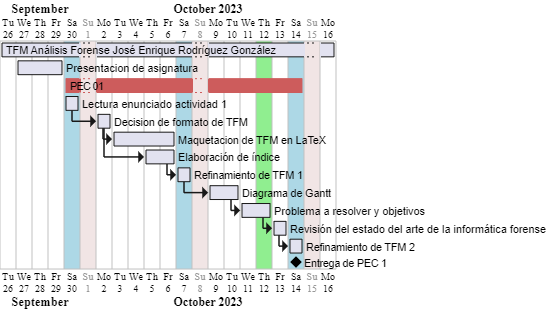
\includegraphics[width=0.8\textwidth]{imagenes/003-diagrama-de-gantt-pec-01.png} 
    \caption{Ejemplo de Diagrama de Gantt relativo al reto/PEC 01.}
    \label{fig:ejemplo_gantt}
\end{figure}

\clearpage

\noindent Relativo al reto/PEC 2 se establece el siguiente diagrama.

\begin{figure}[htp]
    \centering
    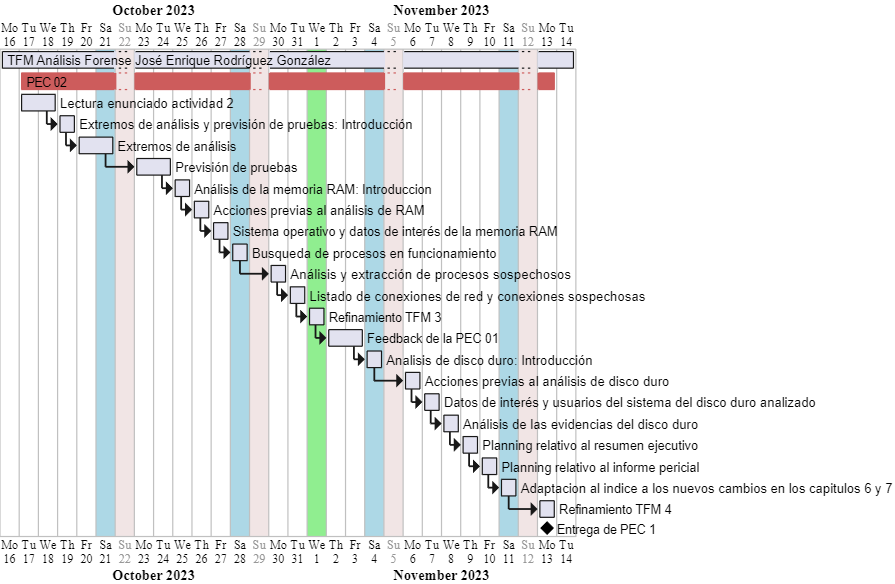
\includegraphics[width=0.8\textwidth]{imagenes/004-diagrama-de-gantt-pec-02.png} 
    \caption{Ejemplo de Diagrama de Gantt relativo al reto/PEC 02.}
    \label{fig:ejemplo_gantt}
\end{figure}

\clearpage

\noindent Relativo al reto/PEC 3 se establece el siguiente diagrama.

\begin{figure}[htp]
    \centering
    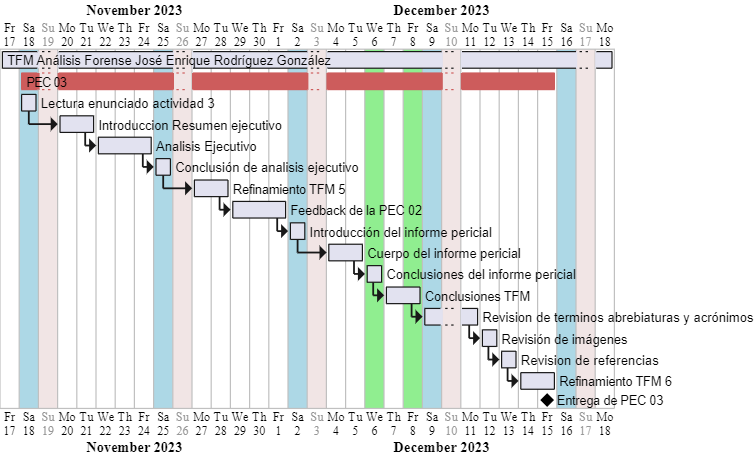
\includegraphics[width=0.8\textwidth]{imagenes/005-diagrama-de-gantt-pec-03.png} 
    \caption{Ejemplo de Diagrama de Gantt relativo al reto/PEC 03.}
    \label{fig:ejemplo_gantt}
\end{figure}


\clearpage

\noindent Relativo al reto/PEC 4 se establece el siguiente diagrama.

\begin{figure}[htp]
    \centering
    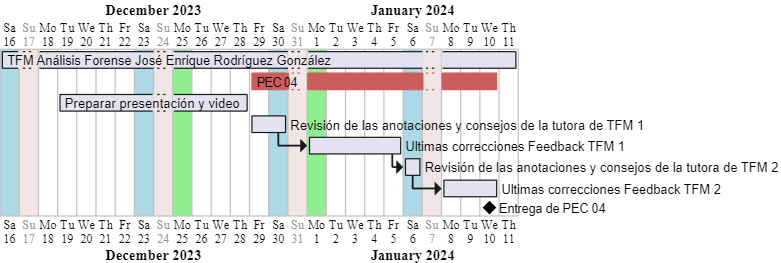
\includegraphics[width=0.8\textwidth]{imagenes/006-diagrama-de-gantt-pec-04.png} 
    \caption{Ejemplo de Diagrama de Gantt relativo al reto/PEC 04.}
    \label{fig:ejemplo_gantt}
\end{figure}


\clearpage

\section{Revisión del estado del arte de la informática forense.}
\subsection{{\color{red}\textbf{DEUDA TÉCNICA: Revisar codigo LaTeX de Estado del arte}}}

\subsection{Introducción}

El análisis forense, también llamado informática forense, computación forense, análisis forense digital o examen forense digital es la aplicación de técnicas científicas y analíticas especializadas a infraestructuras tecnológicas que permiten identificar, preservar, analizar y presentar datos válidos dentro de un proceso legal.

Dichas técnicas incluyen reconstruir elementos informáticos, examinar datos residuales, autenticar datos y explicar las características técnicas del uso de datos y bienes informáticos.

Esta disciplina no sólo hace uso de tecnologías de punta para mantener la integridad de los datos y del procesamiento de los mismos; sino que también requiere de una especialización y conocimientos avanzados de informática y sistemas para identificar lo que ha ocurrido dentro de cualquier dispositivo electrónico. La formación de un informático forense abarca no sólo el conocimiento del software, sino también de hardware, redes, seguridad, piratería, hackeo y recuperación de información.

La informática forense ayuda a detectar pistas sobre ataques informáticos, robos de información, conversaciones o para recolectar evidencias en correos electrónicos y chats.

La evidencia digital o electrónica es sumamente frágil, de ahí la importancia de mantener su integridad; por ejemplo, el simple hecho de pulsar dos veces en un archivo modificaría la última fecha de acceso del mismo.

Dentro del proceso del análisis forense, un examinador forense digital puede llegar a recuperar información que haya sido borrada desde el sistema operativo. El informático forense debe tener muy presente el principio de intercambio de Locard por su importancia en el análisis criminalístico, así como el estándar de Daubert para hacer admisibles en juicio las pruebas presentadas por el experto forense.

Es muy importante mencionar que la informática o el análisis forense no tiene como objetivo prevenir delitos, por lo que resulta imprescindible tener claros los distintos marcos de actuación de la informática forense, la seguridad informática y la auditoría informática.

\subsection{Deficiniciones.}

Existen diferentes términos referentes a la ciencia forense en informática. Cada uno de estos términos trata de manera particular o general temas que son de interés para las ciencias forenses.

\begin{itemize}
    \item \textbf{Computación forense (computer forensics):}
    \begin{itemize}
        \item Disciplina de la ciencia forense que considera los procedimientos en relación con las evidencias para descubrir e interpretar la información en los medios informáticos con el fin de establecer hipótesis o hechos relacionados con un caso. (Centrada en las consideraciones forenses).
        \item Disciplina científica que ofrece un análisis de la información que contienen las tecnologías y de los equipos de computación a partir de su compresión.(Centrada en la tecnología).
    \end{itemize}
    \item \textbf{Ciencia forense en las redes (network forensics):}
    \begin{itemize}
        \item Trata las operaciones de redes de computadores, estableciendo rastros e identificando movimientos y acciones. Es necesario entender los protocolos, configuraciones y la infraestructura de las comunicaciones. A diferencia de la computación forense, es necesario poder establecer relaciones entre eventos diferentes e incluso aleatorios.
    \end{itemize}
    \item \textbf{Ciencia forense digital (digital forensics):}
    \begin{itemize}
        \item Es una forma de aplicar los conceptos y procedimientos de la criminalística a los medios informáticos o digitales. Su objetivo es apoyar al poder judicial en el contexto de la inseguridad informática es decir, la perpetración de posibles delitos aclarando temas relacionados con incidentes o fraudes.
    \end{itemize}
\end{itemize}

\subsection{Objetivos de la informática forense.}

La informática forense tiene tres objetivos:

- La compensación de los daños causados por los intrusos o criminales.

- La persecución y procesamiento judicial de los criminales.

- La creación y aplicación de medidas para prevenir casos similares.

Estos objetivos se alcanzan de varias formas, siendo la principal la recopilación de evidencias.

Es importante mencionar que quienes se dedican a la informática forense deben ser profesionales con altos niveles de ética, pues gracias a su trabajo se toman decisiones sobre los hechos y casos analizados.

\subsection{Evidencia digital.}

Los discos duros, las memorias USB y las impresoras (entre otros elementos) se pueden considerar evidencias en un proceso legal, al igual que las huellas digitales o las armas. Las evidencias digitales son las que se extraen de un medio informático.

\textbf{Características.}

Estas evidencias comparten una serie de características que dificultan el ejercicio de la computación forense:

1. Volatilidad.

2. Anonimato.

3. Facilidad de duplicación.

4. Alterabilidad.

5. Facilidad de eliminación.

\textbf{Categorías.}

Estas evidencias se pueden dividir en tres categorías:

1. Registros almacenados en el equipo de tecnología informática (ej. imágenes y correos).

2. Registros generados por equipos de tecnología informática (ej. transacciones, registros en eventos).

3. Registros parcialmente generados y almacenados en los equipos de tecnología informática (ej. consultas en bases de datos).

\textbf{Dispositivos a analizar.}

Cualquier infraestructura informática que tenga una memoria (almacenamiento) es susceptible a los análisis:

\begin{itemize}
    \item Disco duro de una Computadora o Servidor.
    \item Documentación referente al caso.
    \item Tipo de sistema de telecomunicaciones.
    \item Dirección MAC.
    \item Inicios de sesiones.
    \item Información de los cortafuegos.
    \item IP, redes Proxy. LMhost, host, conexiones cruzadas, pasarelas.
    \item Software de supervisión y seguridad.
    \item Credenciales de autentificación.
    \item Rastreo de paquetes de red.
    \item Teléfonos móviles o celulares (telefonía móvil)
    \item Agendas electrónicas (PDA).
    \item Dispositivos de GPS.
    \item Impresoras.
    \item Memorias USB.
    \item BIOS.
\end{itemize}

\subsection{Perspectiva de tres roles.}

En el análisis de un caso en el que sea necesario el cómputo forense, hay tres roles principales que son importantes y se deben tener en cuenta: el intruso, el administrador y la infraestructura de la seguridad informática, al igual que el investigador.

\textbf{Intrusos}

El intruso es aquel que ataca un sistema, hace cambios no autorizados, manipula contraseñas o cambia configuraciones, entre otras actividades que ponen a prueba la seguridad de un sistema. La intención de los intrusos es un punto clave para poder analizar el caso, ya que no se puede comparar un intruso cuya motivación es el dinero con otro cuya motivación es la demostración de sus habilidades. Jeimy J. Cano hace una comparación entre las motivaciones de diferentes tipos de atacantes, basada en el artículo de Steven Furnell, Cybercrime.

En la primera fase (reconocimiento), se busca reconocer y recolectar información. De esta manera, el atacante puede saber cómo puede actuar y los riesgos posibles, para así poder avanzar. En la segunda fase (ataque) se compromete el sistema, avanzando hasta el nivel más alto, teniendo el control del sistema atacado. Esta etapa usualmente se maneja de manera discreta, lo que dificulta la identificación del intruso. Usualmente, la vanidad del intruso y la falta de discreción ayudan al investigador a resolver el caso con mayor facilidad. Finalmente, (en la fase de eliminación) se altera, elimina o desaparece toda la evidencia que pueda comprometer al intruso en algún caso judicial. Del cuidado con el que el atacante proceda en esta fase depende el proceso del informático forense y del caso.

\textbf{Administradores y la infraestructura de la seguridad informática}

El administrador del sistema es el experto encargado de la configuración de este, de la infraestructura informática y de la seguridad del sistema. Estos administradores son los primeros en estar en contacto con la inseguridad de la información, ya sea por un atacante o por una falla interna de los equipos. Al ser los arquitectos de la infraestructura y de la seguridad de la información del sistema, son quienes primero deberían reaccionar ante un ataque. Además, ellos deben proporcionar su conocimiento de la infraestructura del sistema para apoyar el caso y poder resolverlo con mayor facilidad.

Las infraestructuras de seguridad informática (realizadas por el administrador) han avanzado a medida que avanzan las tecnologías. Inicialmente, se utilizaba una infraestructura centralizada en la cual la información se encontraba en un equipo. Por lo tanto, en este caso la seguridad informática se concentraba en el control del acceso a los equipos con la información, al control del lugar en donde se encontraban y en el entrenamiento de quienes estaban encargados de manejar los equipos. Pero con la tecnología fueron cambiando las infraestructuras y las inseguridades cambiaron. Así es como se crearon los proxies, firewall, el sistema de detección de intrusos (IDS) , el sistema de prevención de intrusos (IPS) entre muchas otras herramientas para proveer una mejor seguridad a los sistemas, ya que ahora el acceso no ocurría solo a través de la máquina, sino a través de otras y de la Web.6

Por otro lado, es importante hablar de la auditabilidad y trazabilidad, que son propiedades del sistema, relacionados con la infraestructura que son útiles como evidencia para el investigador. La auditabilidad es la capacidad del sistema para registrar los eventos de una acción en particular con el fin de mantener la historia de estos y de realizar un control con mayor facilidad. En cambio, la trazabilidad es la propiedad que tiene un sistema para rastrear o reconstruir relaciones entre diferentes objetos monitoreados.6

Es importante resaltar que el administrador debe conocer lo suficiente sobre la infraestructura del sistema para poder colaborar con el caso, ya que su análisis puede facilitar el proceso del investigador forense. Adicionalmente, contar con los rastros y registro de eventos (Auditoría informática) en los sistemas es crucial para el administrador y su infraestructura, no solo porque genera confianza en sus clientes, sino también porque es una buena práctica en términos de seguridad para toda la empresa.

\textbf{Investigador}

Es un nuevo profesional que actúa como experto, criminalista digital, o informático. Comprende y conoce las nuevas tecnologías de la información. Además, el investigador analiza la inseguridad informática emergente en los sistemas. El perfil del investigador es nuevo y necesario en el contexto abierto informático en el que vivimos. Por lo tanto, es necesario formar personas que puedan trabajar como investigadores en la disciplina emergente de la criminalística digital y el cómputo forense. Estas prácticas emergentes buscan articular las prácticas generales de la criminalística con las evidencias digitales disponibles en una escena del crimen. El trabajo del informático es indagar en las evidencias, analizarlas y evaluarlas para poder decidir cómo estas evidencias pueden ayudar a resolver el caso. Por lo tanto, es ideal que un investigador tenga conocimientos (al menos) sobre las siguientes áreas: justicia criminal, auditoría, administración y operación de tecnologías de Información.

En una investigación informática forense, hay ocho roles principales en un caso: el líder del caso, el propietario del sistema, el asesor legal, el auditor/ingeniero especialista en seguridad de la información, el administrador del sistema, el especialista en informática forense, el analista en informática forense y el fiscal. Usualmente, entre todos estos roles, los informáticos forenses pueden tomar los siguientes cuatro roles:

- Líder del caso: es aquel que planea y organiza todo el proceso de investigación digital. Debe identificar el lugar en donde se realizará la investigación, quienes serán los participantes y el tiempo necesario para esta.

- Auditor/ingeniero especialista en seguridad de la información: conoce el escenario en donde se desarrolla la investigación. Tiene el conocimiento del modelo de seguridad, los usuarios y las acciones que pueden realizar en el respectivo sistema. A partir de sus conocimientos debe entregar información crítica a la investigación.

- Especialista en informática forense: es un criminalista digital que debe identificar los diferentes elementos probatorios informáticos vinculados al caso, determinando la relación entre los elementos y los hechos para descubrir el autor del delito.

- Analista en informática forense: examina en detalle los datos, los elementos informáticos recogidos en la escena del crimen con el fin de extraer toda la información posible y relevante para resolver el caso.


\subsection{Pasos del proceso del cómputo forense.}

A continuación se describe el proceso de análisis forense:

\textbf{Identificación}

Es muy importante conocer los antecedentes a la investigación "HotFix", la situación actual y el proceso que se quiere seguir para poder tomar la mejor decisión con respecto a las búsquedas y las estrategias (debes estar bien programado y sincronizado con las actividades a realizar, herramientas de extracción de los registros de información a localizar). Incluye muchas veces (en un momento específico observar, analizar e interpretar y aplicar la certeza, esto se llama criterio profesional que origina la investigación) la identificación del bien informático, su uso dentro de la red, el inicio de la cadena de custodia (proceso que verifica la integridad y manejo adecuado de la evidencia), la revisión del entorno legal que protege el bien y del apoyo para la toma de decisión con respecto al siguiente paso una vez revisados los resultados.

\textbf{Preservación}

Este paso incluye la revisión y generación de las imágenes forenses de la evidencia para poder realizar el análisis. Esta duplicación se realiza utilizando tecnología punta para poder mantener la integridad de la evidencia y la cadena de custodia requerida (soportes). Al realizar una imagen forense, nos referimos al proceso que se requiere para generar una copia “bit-a-bit” (copia binaria) de todo el disco duro, el cual permitirá recuperar (en el siguiente paso) toda la información contenida y borrada del disco duro. Para evitar la contaminación del disco duro, normalmente se ocupan bloqueadores de escritura de hardware, los cuales evitan el contacto de lectura con el disco, lo que provocaría una alteración no deseada en los medios.

\textbf{Análisis}

Proceso de aplicar técnicas científicas y analíticas a los medios duplicados por medio del proceso forense para poder encontrar pruebas de ciertas conductas. Se pueden realizar búsquedas de cadenas de caracteres, acciones específicas del o de los usuarios de la máquina como son el uso de dispositivos de USB (marca, modelo), búsqueda de archivos específicos, recuperación e identificación de correos electrónicos, recuperación de los últimos sitios visitados, recuperación de la caché del navegador de Internet, etc.

\textbf{Presentación}

Es la recopilación de toda la información que se obtuvo a partir del análisis para realizar el reporte y la presentación a los abogados, jueces o instancias que soliciten este informe, la generación (si es el caso) de una pericial y de su correcta interpretación sin hacer uso de tecnicismos; se deberá presentar de manera cauta, prudente y discreta al solicitante la documentación, ya que siempre existirán puertas traseras dentro del sistema en observación. Debe ser muy específica la investigación dentro del sistema que se documenta porque se compara y vincula una plataforma de telecomunicación y cómputo forense que están muy estrechamente enlazadas, sin olvidar los medios de almacenamiento magnéticos portables basados en software libre y privativo. La información que se transmite debe manejarse con cuidado, porque el prestigio técnico depende de las plataformas y los sistemas

Para poder realizar con éxito su trabajo, el investigador nunca debe olvidar:

- Ser imparcial. Solamente analizar y reportar lo encontrado.

- Realizar una investigación formal sin conocimiento y experiencia.

- Mantener la cadena de custodia (proceso que verifica la integridad y manejo adecuado de la evidencia).

- Documentar toda actividad realizada.

El especialista debe conocer también sobre:

- Desarrollo de los exploit (vulnerabilidades), esto le permite al informático forense saber qué tipo de programas se pondrán de moda, para generar una base de estudio que le permita observar patrones de comportamiento.


\subsection{Retos y riesgos en el cómputo forense.}

Al estar en un escenario que evoluciona constantemente, cada vez surgen más retos y riesgos en el área de la informática forense. Entre ellos la formación de informáticos forenses, la confiabilidad de las herramientas, la facilidad de la destrucción de las evidencias, las amenazas estratégicas y tácticas que plantea el ciberterrorismo; y las tecnologías emergentes como la nube, las tecnologías móviles, y las redes sociales. Algunos de estos temas se abordarán a continuación:

\textbf{Formación de informáticos forenses}

Los criminales informáticos son una nueva generación de delincuentes, en este contexto, es necesario desarrollar un nuevo tipo de investigadores: los informáticos forenses. En este momento es un desafío encontrar personas que tengan este perfil, ya que no existen suficientes programas que realicen este tipo de formación. Adicionalmente, en este momento, la mayoría de las personas ignoran la importancia de los informáticos forenses porque no son conscientes de la dimensión del cibercrimen. Usualmente se cree que no es algo tan grave y se le da mayor importancia a otro tipo de crímenes.

Por lo tanto, se deben plantear programas e iniciativas para poder realizar esta formación. Según investigaciones e iniciativas ya realizadas, hay cuatro componentes principales que deben estar presentes en un programa de computación forense o forensia digital: contenido multidisciplinario, ejercicios prácticos, profesores de calidad y ejemplos del mundo real (investigación de Taylor Endicott-Popovsky y Phillips, 2007).

\begin{itemize}
    \item \emph{Contenido multidisciplinario:} técnico en informática, conocimiento de criminalística, seguridad y delitos informáticos, entre otros.
    \item \emph{Ejercicios prácticos en el laboratorio:} con herramientas tecnológicas forenses, en diferentes niveles de dificultad y variedad de componentes a analizar.
    \item \emph{Profesores calificados:} con alto conocimiento en el tema.
    \item \emph{Ejemplos del mundo real:} con el fin de dar mayor profundidad al aprendizaje.
\end{itemize}



\textbf{Confiabilidad de las herramientas}

Las herramientas existentes disponibles para el cómputo forense presentan otro reto. Las herramientas licenciadas exigen a los investigadores inversiones altas (tanto en hardware, como en software), al adquirirlas y para mantenerlas. Adicionalmente, como las herramientas están avanzando constantemente requieren técnicos y usuarios que estén constantemente aprendiendo las actualizaciones, las modificaciones y los posibles errores. Por otro lado, las herramientas de código abierto son cuestionadas en muchos tribunales por su confiabilidad. Por lo tanto, no se recomiendan a la hora de usarse en una audiencia.

Es por esto que el NIST (National Institute of Standards and Technlogy de Estados Unidos) ha planteado importantes investigaciones para probar y poner reglas para las herramientas del cómputo forense, en su proyecto NIST Computer Forensic Tool Testing Program. Las pruebas realizadas serán útiles para cumplir las exigencias del test de Daubert standard, prueba que establece la confiabilidad de las herramientas en computación forense

\subsection{Herramientas de Analisis Forense.}

La siguiente tabla compara cuatro herramientas reconocidas internacionalmente al ser muy completas. Luego, se encuentra una lista más completa de herramientas útiles para la labor del investigador.


\begin{table}[h!]
    \centering
    \caption{Comparativa de herramientas forenses}
    \begin{tabular}{|l|c|c|c|c|}
        \hline
        Herramienta & Licencia & Imagen & Control de Integridad & Administración del caso \\
        \hline
        Encase & SÍ & SÍ & SÍ & SÍ \\
        \hline
        Forensic Toolkit & SÍ & SÍ & SÍ & SÍ \\
        \hline
        Winhex & SÍ & SÍ & SÍ & SÍ \\
        \hline
        Sleuth Kit & NO & SÍ & SÍ & SÍ \\
        \hline
    \end{tabular}
    \label{table:comparativa_herramientas}
\end{table}

\begin{itemize}
    \item Air (Forensics Imaging GUI).
    \item Autopsy (Forensics Browser for Sleuth Kit)Cryptcat (Command Line)Deep Freeze.
    \item Dcfldd (DD Imaging Tool command line tool and also works with AIR).
    \item Dumpzilla (Forensics Browser: Firefox, Iceweasel and Seamonkey).
    \item Encase: \url{https://www.guidancesoftware.com/encase-forensic?cmpid=nav_r}
    \item Exif Viewer (Visor de metadatos en imágenes).
    \item Faces.
    \item Foremost (Data Carver command line tool).
    \item Forensik Toolkit: \url{https://accessdata.com/products-services/forensic-toolkit-ftk}.
    \item Helix.
    \item Hetman software (Recuperador de datos borrados por los criminales).
    \item Hiren´s boot.
    \item Md5deep (MD5 Hashing Program).
    \item Metashield Analyser Online (Analizador de metadatos online).
    \item Mini XP.
    \item NTFS-Tools.
    \item Netcat (Command Line).
    \item Net resident.
    \item NetFlow.
    \item Py-Flag (Forensics Browser).
    \item Qtparted (GUI Partitioning Tool).
    \item R-Studio Emergency (Bootable Recovery media Maker).
    \item R-Studio Network Edtion.
    \item R-Studio RS Agent.
    \item Regviewer (Windows Registry).
    \item Sleuth Kit (Forensics Kit. Command Line): \url{https://www.sleuthkit.org/}.
    \item Snort.
    \item Viewer.
    \item Volatility (Reconstrucción y análisis de memoria RAM).
    \item X-Ways Forensics.
    \item X-Ways WinHex \url{https://www.x-ways.net/winhex/}.
    \item X-Ways WinTrace.
\end{itemize}


\noindent \textbf{Herramientas para el análisis de discos duros}

\begin{itemize}
    \item AccessData Forensic ToolKit (FTK).
    \item Guidance Software EnCase.
    \item Kit Electrónico de Transferencia de datos.
\end{itemize}

\noindent \textbf{Herramientas para el análisis de correos electrónicos}

\begin{itemize}
    \item Paraben
    \item AccessData Forensic ToolKit (FTK)
\end{itemize}

\noindent \textbf{Herramientas para el análisis de dispositivos móviles}

\begin{itemize}
    \item Cellebrite UFED Touch 2, Physical Analyzer.
    \item AccessData Mobile Phone Examiner Plus (MPE+)
\end{itemize}

\noindent \textbf{Herramientas para el análisis de redes}

\begin{itemize}
    \item E-Detective - Decision Computer Group
    \item SilentRunner - AccessData
    \item NetworkMiner
    \item Netwitness Investigator
\end{itemize}

\noindent \textbf{Herramientas para filtrar y monitorear el tráfico de una red tanto interna como a internet}

\begin{itemize}
    \item Tcpdump
    \item USBDeview
    \item SilentRunner - AccessData
    \item WireShark
\end{itemize}

\noindent \textbf{Términos importantes}

\begin{itemize}
    \item \emph{Cadena de custodia:} la identidad de personas que manejan la evidencia en el tiempo del suceso y la última revisión del caso. Es la responsabilidad de la persona que maneja la evidencia asegurar que los artículos son registrados y contabilizados durante el tiempo en el cual están en su poder, y que son protegidos, así mismo llevando un registro de los nombres de las personas que manejaron la evidencia o artículos durante el lapso de tiempo y fechas de entrega y recepción.
    \item \emph{Imagen forense:} técnica llamada también "espejeo" (en inglés "Mirroring"), la cual es una copia binaria de un medio electrónico de almacenamiento. En la imagen quedan grabados los espacios que ocupan los archivos y las áreas borradas incluyendo particiones escondidas.
    \item \emph{Análisis de archivo:} examina cada archivo digital descubierto y crea una base de datos de información relacionada al archivo (metadatos, etc.), consistente entre otras cosas en la firma del archivo o hash (indica la integridad del archivo).
\end{itemize}

{\color{red}\textbf{DEUDA TÉCNICA: Revisar codigo LaTeX de Estado del arte}}
{\color{red}\textbf{DEUDA TÉCNICA: plantear posible reducción del estado del arte}}
{\color{red}\textbf{DEUDA TÉCNICA: Referencia a WIKIPEDIA}}
\clearpage

\chapter{Extremos del análisis y previsión de pruebas técnicas.}
En la era digital actual, la capacidad de llevar a cabo análisis forenses en ordenadores se ha convertido en una competencia crítica dentro del ámbito de la investigación criminal. El análisis forense informático permite a los investigadores descubrir, preservar y analizar datos en dispositivos electrónicos que pueden ser críticos para resolver delitos. Este capítulo se dedica al estudio meticuloso de los métodos y prácticas estándar en la computación forense, con un enfoque específico en la adquisición y análisis de datos de la memoria RAM y discos duros. Se expondrá la metodología utilizada para garantizar la integridad de la evidencia y se ilustrarán los desafíos asociados a la recolección y el análisis de datos digitales.

Con el avance de la tecnología, los investigadores forenses enfrentan la dualidad de oportunidades y desafíos. Por un lado, las herramientas modernas ofrecen capacidades sin precedentes para recuperar y analizar datos; por otro lado, la creciente sofisticación del software y hardware supone nuevos niveles de complejidad y la necesidad de constante actualización en conocimientos y técnicas. Este capítulo también contempla la noción de deuda técnica asociada a la utilización de herramientas y sistemas operativos en la investigación forense, reconociendo la importancia de mantener un enfoque crítico hacia las herramientas utilizadas.

La documentación y control de versiones son aspectos cruciales en cualquier proyecto de investigación y desarrollo, más aún en el ámbito forense digital, donde la transparencia y reproducibilidad son fundamentales. Se detallará el uso del repositorio de Github (https://github.com/jrodg85/TFM-ANALISIS-FORENSE) para la documentación del TFM y el control de versiones aplicado al proceso de análisis forense. Se discutirá la relevancia de la colaboración y el seguimiento preciso de cambios en el código y documentos relacionados con el proyecto.

Finalmente, no se puede ignorar el papel fundamental que juega el acceso a recursos online en la actualización constante y el acceso a información relevante y actualizada en el campo de la forense digital. La Internet es una fuente inagotable de conocimiento, pero también presenta riesgos que deben ser gestionados con prudencia. En resumen, este capítulo traza el panorama del análisis forense en ordenadores, describiendo las herramientas y metodologías utilizadas, así como las mejores prácticas en la documentación y gestión de la información digital en investigaciones forenses.

Esta introducción proporciona una vista general y establece las expectativas para el contenido que seguirá, preparando al lector para los detalles técnicos y metodológicos que se presentarán en el capítulo.
\clearpage

\section{Propuesta de extremos.}
La presente investigación tiene como propósito fundamental el establecimiento de un marco metodológico para el análisis forense de ordenadores, específicamente orientado hacia la identificación, recolección y análisis de evidencias digitales que puedan ser presentadas en un entorno judicial. A continuación, se delinean los extremos de esta propuesta:

\textbf{Objeto de Estudio:}

\begin{itemize}
  \item La investigación se centrará exclusivamente en el análisis forense del material facilitado para el desarrollo de la asignatura por parte del profesorado de la asignatura.
  \item Se realizará una breve indicacion sobre la aplicacion utilizada con cada uno de los objetivos del presente TFM.
\end{itemize}


\textbf{Alcance metodológico:}

\begin{itemize}
  \item La validación de la integridad de la evidencia se hará mediante el uso de funciones hash estándar.
  \item Se examinarán las metodologías para el análisis de la memoria volátil y no volátil.
\end{itemize}


\textbf{Limitaciones:}

\begin{itemize}
  \item La validación de la integridad de la evidencia se hará mediante el uso de funciones hash estándar.
  \item Se examinarán las metodologías para el análisis de la memoria volátil y no volátil.
\end{itemize}


\textbf{Exclusiones:}

\begin{itemize}
  \item No se utilizará material de análisis que no sea el proporcionado por la asignatura.
\end{itemize}



\clearpage

\section{Previsión de pruebas técnicas.}
\textbf{Pruebas técnicas:}

\begin{itemize}
    \item El propósito de estas pruebas técnicas es lo indicado en el apartado de problema a resolver del presente Trabajo de fin de master
    \begin{itemize}
        \item Solventar las necesidades del gerente de la empresa mediante el análisis forense del disco duro y la captura de memoria de un ordenador personal, en un caso real con un sistema virtualizado.
        \item Posible vinculación con una presunta conducta delictiva real.
    \end{itemize}
    \item Importancia de las pruebas para validar la hipótesis y objetivos de investigación.
    \begin{itemize}
        \item La posible imputación de los hechos ocurridos y tomar posibles medidas legales contra el autor univoco de la acción detectada.
    \end{itemize}
\end{itemize}

\textbf{Marco metodológico de las pruebas:}

\begin{itemize}
    \item Las pruebas que se realizarán serán una investigación y un estudio temporal de los hechos ocurridos dentro del pc.
    \item Se emplearán herramientas de análisis forense en sus distintos sistemas operativos (Linux/Windows) para su detección.
    \item se tratará de arrancar el sistema virtualizado para posible carving de la información del disco duro por posible eliminación de pruebas por parte del posible infractor.
    \item La planificación de las pruebas ha quedado detallado en la sección "planificación temporal de las tareas".
\end{itemize}


\textbf{Criterios de éxito de las pruebas:}






\clearpage

\chapter{Análisis de la memoria RAM.}
El análisis forense de la memoria RAM es un componente crítico en la investigación digital, pues permite a los analistas extraer información valiosa que no persiste una vez que el dispositivo se apaga. Esta volatilidad hace que la memoria RAM sea una fuente de evidencia esencial, especialmente en casos donde los procesos activos y la información en tránsito son relevantes para el caso. El presente capítulo detalla un enfoque metodológico estructurado para examinar de manera exhaustiva el contenido de la memoria RAM capturada de un sistema informático, con el objetivo de identificar y analizar aspectos críticos que contribuyan a la investigación.

Las acciones específicas que se abordarán son las siguientes:

\begin{enumerate}
    \item  \textbf{Comprobación del MD5:}

    Iniciaremos con la verificación de la integridad del volcado de la memoria RAM mediante el cálculo de su suma de verificación MD5. Este paso es fundamental para asegurar que los datos analizados no han sido alterados desde el momento de su adquisición, garantizando así la cadena de custodia digital.

    \item \textbf{Identificación del Sistema Operativo:}

    Aunque ya intuyamos, por el apartado anterior datos básicos del Sistema operativo, es vital determinar la versión y configuración del sistema operativo en uso, ya que esto influirá en la interpretación de los datos y en la selección de las herramientas de análisis adecuadas.

    \item \textbf{Búsqueda de Datos de Interés:}

    Seguiremos con la inspección minuciosa del contenido de la memoria para identificar información potencialmente relevante para el caso. Esto incluye, pero no se limita a, datos residuales de aplicaciones, fragmentos de comunicaciones y elementos que puedan ser reconstruidos para obtener evidencia. Servirá para tener una previsión de por donde dirigir el estudio de todo el análisis forense.


    \item \textbf{Búsqueda de Procesos en Funcionamiento de Interés:}

    Un punto focal de nuestra investigación será el examen de los procesos activos en el momento de la captura de la memoria. Esta inspección nos permitirá comprender mejor el estado del sistema antes del apagado o la hibernación.

    \item \textbf{Análisis y Extracción de Procesos Sospechosos:}

    Finalmente, nos concentraremos en reconstruir y examinar las conexiones de red activas y pasivas. El objetivo es identificar patrones de tráfico inusuales o conexiones que puedan indicar comunicación con servidores de comando y control, exfiltración de datos o cualquier otra actividad que se considere sospechosa.

\end{enumerate}

El resultado de este análisis exhaustivo proporcionará una comprensión detallada de lo que estaba ocurriendo en el sistema en el momento de la captura de la memoria. Esta información es invaluable para formar una imagen completa de los eventos bajo investigación y para establecer hechos concretos que puedan ser presentados como evidencia en un entorno judicial.



\clearpage

\section{Acciones previas al análisis de la memoria RAM.}
En el presente TFM, se nos ha proporcionado a los alumnos un archivo de captura de memoria RAM .mem. Por otro lado, se nos ha proporcionado los resúmenes o hash en MD5 y en SHA1 de los archivos tal y como se muestra en la siguiente imagen.

\begin{figure}[htp]
    \centering
    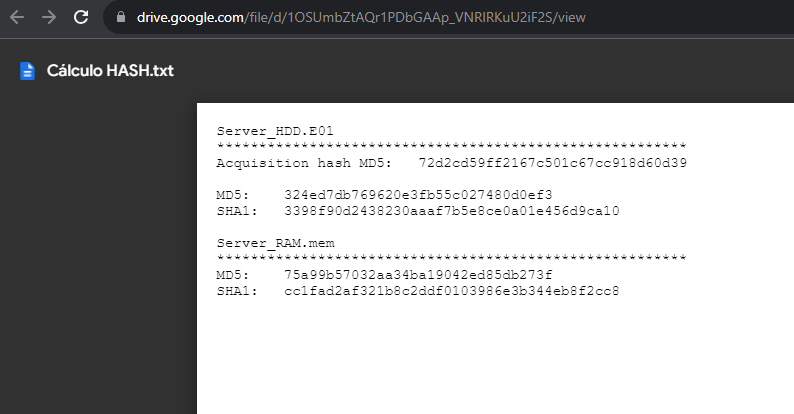
\includegraphics[width=1.0\textwidth]{imagenes/007-imagen-hash-archivos.png}
    \caption{Pantallazo hash imágenes de archivos.}
    \label{Pantallazo hash imágenes de archivos.}
\end{figure}

Como Podemos ver, los hash resúmenes del archivo de la ram, tememos los siguientes hashes en MD5 y en SHA1:

\begin{itemize}
    \item \textbf{MD5:} 75a99b57032aa34ba19042ed85db273f
    \item \textbf{SHA1:} cc1fad2af321b8c2ddf0103986e3b344eb8f2cc8
\end{itemize}

Eñ hash tal y como se indica en los apuntes de la asignatura, en el módulo de Fases y metodología del análisis forense, durante la adquisición de evidencias digitales dice  lo siguiente:

Una vez generada la copia o clon del soporte original, el programa o el dispositivo hardware empleado en este proceso realiza el cálculo del CRC o del valor hash del soporte original y del destino, con la finalidad de garantizar que los dos son idénticos y que la copia se ha producido sin ningún error. Este cálculo puede realizarse sobre todo el conjunto de información contenida en el soporte original, o bien emplear solamente un conjunto de ficheros del total.

A su vez, en el glosario de términos la definición de hash es la siguiente:

Es una función matemática unidireccional que resume un mensaje de tamaño variable (por ejemplo, un archivo), en una representación de tamaño fijo. Es poco probable que dos ficheros distintos tengan la misma representación hash, lo cual significa que este valor puede utilizarse a efectos de comprobación de la integridad de un archivo (o de un sistema entero). Las funciones hash más conocidas son MD5 y SHA-1.

Una vez descargado el archivo de captura de la memoria RAM, procedemos a usar PowerShell para determinar el hash del archivo. Para ello usamos el comando  Get-FileHash [Argumento] -Algorithm MD5. En nuestro caso hemos usado los siguientes comandos:


\begin{verbatim}
Get-FileHash .\Server_RAM.mem -Algorithm MD5
\end{verbatim}


\begin{verbatim}
Get-FileHash .\Server_RAM.mem -Algorithm SHA1
\end{verbatim}



La respuesta de PowerShell es el siguiente respectivamente

\begin{verbatim}
Algorithm       Hash                                                                   Path
---------       ----                                                                   ----
MD5             75A99B57032AA34BA19042ED85DB273F                                       D:\TFM\RAM\...
\end{verbatim}

\begin{verbatim}
Algorithm       Hash                                                                   Path
---------       ----                                                                   ----
SHA1            CC1FAD2AF321B8C2DDF0103986E3B344EB8F2CC8                               D:\TFM\RAM\...
\end{verbatim}

Se puede observar en la siguiente imagen la respuesta de PowerShell de los hashes de MD5 y SHA1.

\begin{figure}[htp]
    \centering
    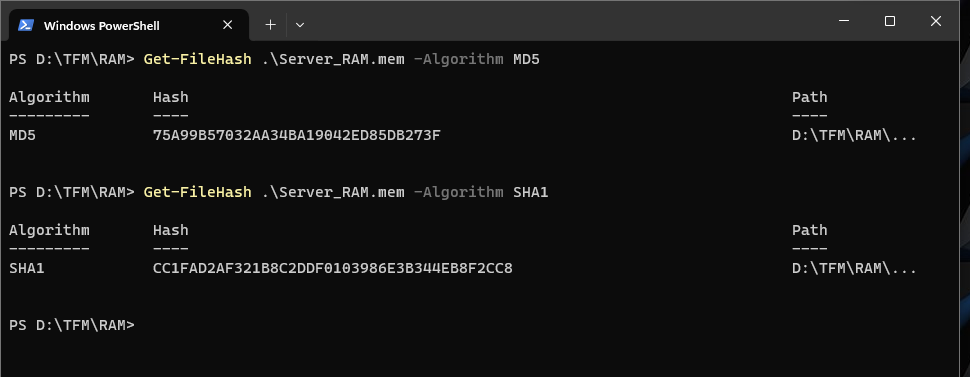
\includegraphics[width=1.0\textwidth]{imagenes/008-captura-hash-PowerShell.png}
    \caption{Hash Ram en PowerShell.}
    \label{Hash Ram en PowerShell.}
\end{figure}

Como conclusión podemos verificar que la integridad de la copia facilitada para realizar el TFM no ha sido vulnerada.
\clearpage

\section{Datos de interés de la captura de la memoria RAM.}
\input{chapter/004-analisis-de-la-memoria-ram/sections/004-03-datos-de-interes-de-la-memoria-ram.tex}
\clearpage

\section{Sistema Operativo de la memoria RAM analizada.}
Procedemos a preparar una máquina virtual con Ubuntu 22.04, el cual le instalamos el volatility según en el siguiente enlace:

\begin{itemize}
    \item https://www.youtube.com/watch?v=5-2-ORNC8CA
\end{itemize}

A continuación procedemos a buscar el perfil con volatility con el comando imageinfo.

\begin{figure}[htp]
    \centering
    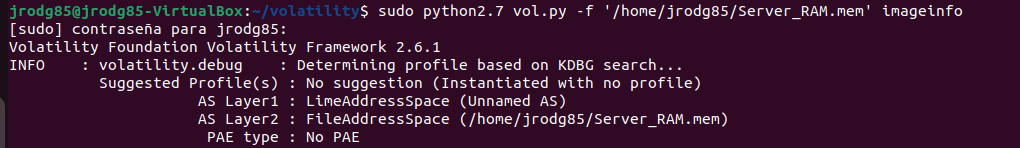
\includegraphics[width=1.0\textwidth]{imagenes/009-captura-imgeinfo.png}
    \caption{captura imageinfo}
    \label{captura imageinfo.}
\end{figure}

Como se puede observar en la imagen anterior, no hemos llegado a encontrar un perfil concreto con imageinfo, eso se debe a que el perfil creado no es el que se encuentra dentro de las conocidas en la base de datos de volatility. Por ello procedemos a buscar dentor de la memoria RAM un string que tenga la cadena de texto "linux version". para ello ejecutamos el comando $strings Server_{RAM}.mem \mid grep -Ei linux version \mid uniq$.

\begin{figure}[htp]
    \centering
    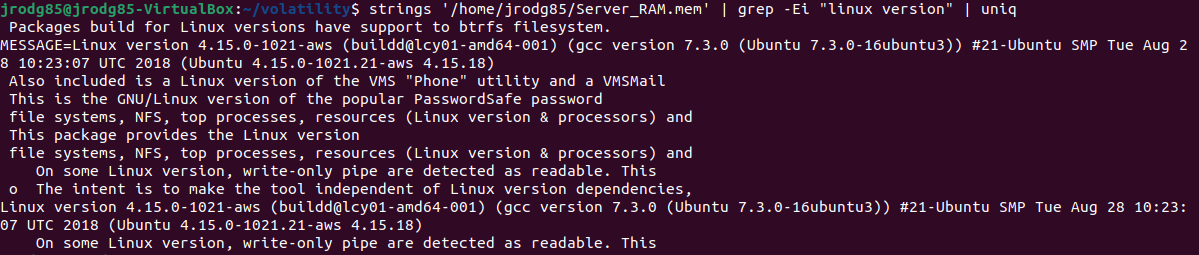
\includegraphics[width=1.0\textwidth]{imagenes/010-buscar-strings-linux-verison.png}
    \caption{captura imageinfo}
    \label{captura linux version.}
\end{figure}


Podemos observar en la imagen anterior que el sistema operativo que utiliza en nuestro caso es un sistema operativo Linux para Amazon Web Service, concretamente el sistema operativo es el \textbf{4.15.0-1021.21-aws 4.15.18}. Esta version de Linux, es muy usada para las instancias de Amazon Web Services.

Como no tenemos el perfil cargado dentro de volatility, nos va a tocar hacer la tarea de cargar un perfil de este Sistema operativo para poder seguir ejecutando la aplicación volatility.

Buscando en google \textbf{linux version 4.15.0-1021.21-aws volatility}, nos encontramos solo un enlace en internet, el cual es https://lists.ubuntu.com/archives/bionic-changes/2018-August/016183.html, con ello nos encontrábamos con algo que ya se intuía previamente, y es que la versión del server de AWS, es basada en un ubuntu 18.04, ya que la fecha que indica 4.15.18 es una fecha en tipo "d.mm.aa".




\clearpage

\section{Búsqueda de procesos en funcionamiento de interés para el análisis.}
\input{chapter/004-analisis-de-la-memoria-ram/sections/004-04-busqueda-de-procesos-en-funcionamiento-de-interés-para-el-análisis.tex}
\clearpage

\section{Análisis y extracción de procesos sospechosos.}
\input{chapter/004-analisis-de-la-memoria-ram/sections/004-05-Analisis-y-extraccion-de-procesos-sospechosos.tex}
\clearpage

\section{Listado de conexiones de red y conexiones sospechosas.}
\input{chapter/004-analisis-de-la-memoria-ram/sections/004-06-listado-de-conexiones-de-red-y-conexiones-sospechosas.tex}
\clearpage

\chapter{Análisis del disco duro.}
\input{chapter/005-analisis-de-disco-duro/005-analisis-del-disco-duro.tex}
\clearpage

\section{Acciones previas al análisis del disco duro.}
\input{chapter/005-analisis-de-disco-duro/sections/005-01-acciones-previas-al-analisis-de-disco-duro.tex}
\clearpage

\section{Datos de interés del disco duro.}
\input{chapter/005-analisis-de-disco-duro/sections/005-02-datos-de-interes-del-disco-duro.tex}
\clearpage

\section{Usuarios del sistema.}
\input{chapter/005-analisis-de-disco-duro/sections/005-03-usuarios-del-sistema.tex}
\clearpage

\section{Análisis de evidencias del disco duro.}
\input{chapter/005-analisis-de-disco-duro/sections/005-04-analisis-de-evidencias-del-disco-duro.tex}
\clearpage

\chapter{Resumen ejecutivo.}
\input{chapter/006-resumen-ejecutivo/006-resumen-ejecutivo.tex}
\clearpage

\chapter{Informe pericial.}
\input{chapter/007-informe-pericial/007-informe-pericial.tex}
\clearpage

\chapter{Conclusiones.}
\input{chapter/008-conclusiones/008-conclusiones.tex}
\clearpage

\chapter{Anexos.}
\input{chapter/009-anexos/009-anexos.tex}
\clearpage

\section{Glosario de términos y abreviaturas.}
CISO
\clearpage

\section{Imágenes.}
\input{chapter/009-anexos/sections/009-02-imagenes.tex}
\clearpage

\bibliography{referencias}
\input{referencias.bib}
\clearpage


\end{document}
